% This is samplepaper.tex, a sample chapter demonstrating the
% LLNCS macro package for Springer Computer Science proceedings;
% Version 2.21 of 2022/01/12
%
\documentclass[runningheads]{llncs}
%
\usepackage[T1]{fontenc}
% T1 fonts will be used to generate the final print and online PDFs,
% so please use T1 fonts in your manuscript whenever possible.
% Other font encondings may result in incorrect characters.
%
\usepackage{graphicx}
\usepackage{tikz}
\usepackage{verbatim}
\usepackage{fancyvrb}
\usepackage{amsmath}
\usepackage{ulem}
% Used for displaying a sample figure. If possible, figure files should
% be included in EPS format.
%
% If you use the hyperref package, please uncomment the following two lines
% to display URLs in blue roman font according to Springer's eBook style:
\usepackage{color}
%\renewcommand\UrlFont{\color{blue}\rmfamily}
%\urlstyle{rm}

\usepackage[utf8]{inputenc}
\usepackage[a4paper,margin=2.5cm]{geometry}

%
\setcounter{tocdepth}{2}
\begin{document}


%\section*{Outline of Changes}

\begin{itemize}
  \item Added a textual example to the introduction.
  \item Added a TikZ diagram to the introduction to illustrate the motivating example graph and query.
  \item Added a simple TikZ diagram illustrating nodes, edges, labels, and properties for the property graph model in Section~2.1.
  \item Included a table distinguishing between walks, trails, simple paths, and acyclic paths in Section~2.2 to enhance clarity.
  \item Provided short example queries in GQL, SQL/PGQ, and Cypher in Section~2.3 to offer practical context for graph query languages.
  \item Reworked Section~3 by introducing a consistent running example, streamlining the presentation of the core algebra operators, and adding concrete examples for selection, union, and concatenation.
  \item Improved Section~4 by adding a step-by-step worked example of recursive path construction via repeated concatenation, illustrating how short path fragments generate longer walks, and clarified the distinction between walks, trails, and acyclic paths using the example sequence.
  \item Extended Section~5 by adding a concrete translation of a GQL path pattern into algebraic operators and included an illustrative example showing additional expressiveness beyond GQL/SQL/PGQ through ordering within recursive path construction.
  \item Expanded Section~6 with a more critical discussion of the advantages and limitations of the proposed path algebra relative to relational algebra, automata-theoretic approaches, and semiring frameworks.
  \item Expanded Section~7 by discussing optimization opportunities, implementation challenges, recursive evaluation complexity, scalability, cost-based optimization, and practical adoption in graph database systems.
  \item Added additional literature references and citations throughout to better relate the presented concepts to the broader graph database and query language literature.
\end{itemize}
%
\title{Core Path Algebra for Graph Queries}
%
\titlerunning{Core Path Algebra for Graph Queries}
% If the paper title is too long for the running head, you can set
% an abbreviated paper title here
%
%\author{First Author\inst{1}\orcidID{0000-1111-2222-3333}
\author{A. Nonymous}
%
\authorrunning{A. Nonymous}
% First names are abbreviated in the running head.
% If there are more than two authors, 'et al.' is used.
%
\institute{University of Stuttgart
\email{stxxxxxx@stud.uni-stuttgart.de}}
%
\maketitle              % typeset the header of the contribution
%

\begin{abstract}
Graph databases are well suited for data with many relationships, and path queries are an important part of modern graph query languages. Languages such as GQL and SQL/PGQ provide constructs for finding and manipulating paths, but a common algebraic way of describing these operations is still developing. This paper examines the path algebra proposed by Angles et al. \cite{angles2024path}. The algebra treats paths as first-class query objects and provides operators for selection, union, concatenation, and recursion. The paper explains these operators and shows how they can be used to describe path queries and path semantics found in GQL and SQL/PGQ. It also compares the path algebra with relational algebra, automata-based approaches to regular path queries, and semiring-based models. The comparison shows how the path algebra relates to existing formalisms while focusing specifically on the construction and manipulation of paths. Finally, the paper discusses the strengths and limitations of the algebra, particularly the challenges of efficiently evaluating recursive path queries.

\keywords{Graph Databases \and
Graph Query Languages \and
Path Algebra \and
GQL \and
SQL/PGQ}

\end{abstract}

%
%

\tableofcontents
\newpage

\section{Introduction}

Graph databases have become an important technology for managing highly connected data, with applications in social networks, knowledge graphs, recommendation systems, and biological networks \cite{angles2017foundations,bonifati2018querying}. Unlike relational systems, graph databases treat relationships as first-class elements, which makes them suited for queries that require navigation through connected data.

Modern graph query languages such as Cypher, SPARQL, SQL/PGQ, and GQL provide support for path-oriented queries \cite{angles2017foundations}. Such queries allow users to express reachability, pattern matching, and recursive navigation over graph structures. This makes path queries an important part of graph query languages and raises the question of how such operations can be described in a common algebraic framework.


For example, consider finding all paths between two nodes whose sequence of edge labels consists of one or more \texttt{KNOWS} relationships followed by zero or more \texttt{LIKES} relationships. Such path patterns can be described using regular expressions over edge labels and are common in graph query languages. Classical relational algebra does in contrast not provide a direct operator for recursive path traversal or transitive closure.

To illustrate, consider the following graph:

\begin{figure}[h!]
  \centering
  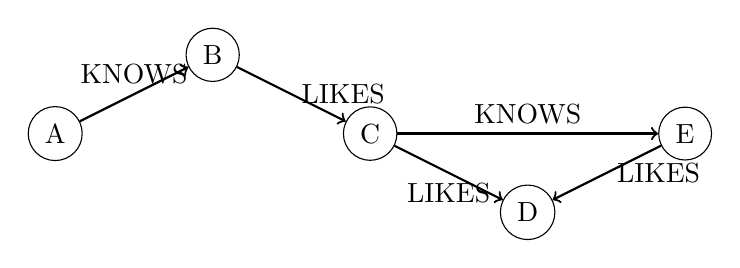
\begin{tikzpicture}
    % Nodes
    \node[circle, draw] (A) at (0,0) {A};
    \node[circle, draw] (B) at (2,1) {B};
    \node[circle, draw] (C) at (4,0) {C};
    \node[circle, draw] (D) at (6,-1) {D};
    \node[circle, draw] (E) at (8,0) {E};

    % Edges
    \draw[->, thick] (A) -- node[midway, above] {KNOWS} (B);
    \draw[->, thick] (B) -- node[midway, right] {LIKES} (C);
    \draw[->, thick] (C) -- node[midway, below] {LIKES} (D);
    \draw[->, thick] (C) -- node[midway, above] {KNOWS} (E);
    \draw[->, thick] (E) -- node[midway, right] {LIKES} (D);
  \end{tikzpicture}
  \caption{Example graph illustrating a path query.}
\end{figure}

In this graph, we seek all paths from node \texttt{A} to node \texttt{D} whose edge-label sequence matches the regular expression

\[
\texttt{KNOWS}^{+}\texttt{LIKES}^{*}.
\]

\[
A \xrightarrow{\texttt{KNOWS}} B
\xrightarrow{\texttt{LIKES}} C
\xrightarrow{\texttt{LIKES}} D
\]

This first path matches the pattern: it contains one \texttt{KNOWS} edge followed by two \texttt{LIKES} edges.

\[
A \xrightarrow{\texttt{KNOWS}} B
\xrightarrow{\texttt{LIKES}} C
\xrightarrow{\texttt{KNOWS}} E
\xrightarrow{\texttt{LIKES}} D
\]

This second path does not match because it contains a \texttt{KNOWS} edge after a \texttt{LIKES} edge.

In graph query languages, such patterns can be expressed using regular path expressions. For example, in GQL-inspired notation one could write:

\begin{Verbatim}
MATCH p = (A)-/:KNOWS+ LIKES*/->(D)
\end{Verbatim}

The essential idea is that the path must match the regular expression \texttt{KNOWS\textsuperscript{+}LIKES\textsuperscript{*}}. The example illustrates why path queries require operations for concatenation and recursion that are not part of classical relational algebra.
Relational algebra provides a foundation for relational query processing and optimization. For graph queries, however, an algebraic foundation for path-based operations is less established, especially when paths themselves are treated as query results.
Angles et al. propose a path algebra in which paths are treated as first-class data objects \cite{angles2024path}. It provides operators for path selection, concatenation, union, and recursion, and is intended to provide an algebraic basis for path queries in graph query languages such as GQL and SQL/PGQ.
This paper examines the core operators of the proposed path algebra and explains how they can be used to represent path queries. It then considers its relationship to relational algebra, automata-based approaches to regular path queries, and semiring-based models for graph problems.
\section{Background}

\subsection{Property Graph Model}

Graph databases are commonly based on the property graph model \cite{angles2018property}. A property graph is a directed, labeled multigraph in which both nodes and edges may carry labels and key-value properties.

Formally, a property graph is defined as a tuple
$G = (N, E, \rho, \lambda, \sigma)$,
where $N$ is the set of nodes, $E$ is the set of edges, $\rho$ defines edge connectivity, $\lambda$ assigns labels, and $\sigma$ defines property mappings \cite{angles2018property}. A path can be represented visually as shown in Figure 2.

\begin{figure}[ht]
    \centering
    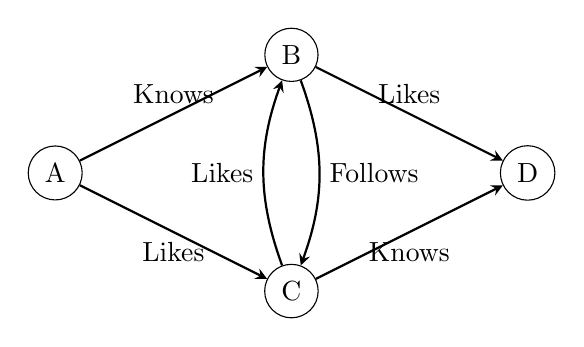
\begin{tikzpicture}[>=stealth]

        % Nodes
        \node[draw, circle] (A) at (0,0) {A};
        \node[draw, circle] (B) at (3,1.5) {B};
        \node[draw, circle] (C) at (3,-1.5) {C};
        \node[draw, circle] (D) at (6,0) {D};

        % Edges
        \draw[->, thick] (A) -- node[above] {Knows} (B);
        \draw[->, thick] (A) -- node[below] {Likes} (C);
        \draw[->, thick] (B) -- node[above] {Likes} (D);
        \draw[->, thick] (C) -- node[below] {Knows} (D);
        \draw[->, thick, bend left=20] (B) to node[right] {Follows} (C);
        \draw[->, thick, bend left=20] (C) to node[left] {Likes} (B);

    \end{tikzpicture}
    \caption{Simple Property Graph Model Illustration}
\end{figure}

\subsection{Paths in Graphs}

A path in a property graph is a sequence of alternating nodes and edges

\[
p = (n_1, e_1, n_2, \dots, e_k, n_{k+1})
\]

such that each edge connects consecutive nodes. Paths may be classified as walks, trails, acyclic paths, or simple paths depending on whether nodes or edges may repeat, as seem in the table below.

Path queries aim to retrieve sets of such paths satisfying structural or label constraints.


\begin{table}[ht]
    \centering
    \begin{tabular}{|l|p{7.5cm}|p{3.2cm}|}
        \hline
        \textbf{Path Type} & \textbf{Description} & \textbf{Example} \\
        \hline
        Walk &
        A path in which nodes and edges may be repeated.
        &
        A $\rightarrow$ B $\rightarrow$ C $\rightarrow$ B $\rightarrow$ D
        \\
        \hline
        Trail &
        A path in which no edge is repeated.
        &
        A $\rightarrow$ B $\rightarrow$ C $\rightarrow$ D
        \\
        \hline
        Acyclic &
        A path in which no node is repeated.
        &
        A $\rightarrow$ B $\rightarrow$ C $\rightarrow$ D
        \\
        \hline
        Simple &
        A path in which no node is repeated, except that the first and last nodes may be the same.
        &
        A $\rightarrow$ B $\rightarrow$ C $\rightarrow$ A
        \\
        \hline
    \end{tabular}
    \caption{Path semantics used in graph query languages \cite{angles2024path}.}
\end{table}

%}

\subsection{Graph Query Languages}

Modern graph query languages such as Cypher, SPARQL, SQL/PGQ, and GQL support path-oriented queries based on regular expressions over edge labels \cite{angles2017foundations,angles2024path}.

In contrast to classical RPQs, these languages aim to return not only reachable node pairs but also the actual witness paths. To control the potentially infinite number of such paths in cyclic graphs, GQL and SQL/PGQ introduce selectors and restrictors, which determine how paths are filtered and how recursion is interpreted \cite{angles2024path}.


\textbf{Example Queries:}

\begin{itemize}

    \item \textbf{Cypher and GQL} -- Matches a \texttt{KNOWS} relationship and returns the path.
\begin{verbatim}
MATCH p = (x)-[:KNOWS]->(y)
RETURN p
\end{verbatim}

    \item \textbf{SQL/PGQ} -- Matches a \texttt{KNOWS} relationship and returns the path.
\begin{verbatim}
SELECT p
FROM GRAPH_TABLE (
  my_graph
  MATCH p = (x)-[:KNOWS]->(y)
  COLUMNS (p)
)
\end{verbatim}

\end{itemize}
%}
\section{Core Path Algebra}

The core idea of the path algebra is to treat paths as first-class data objects, similar to tuples in relational algebra \cite{angles2024path}. The operators take sets of paths as input and return sets of paths, which allows their results to be combined into larger expressions.

\subsection{Core Operators}

The core algebra consists of three fundamental operators \cite{angles2024path}:

\begin{itemize}
    \item \textbf{Selection} ($\sigma$): filters paths based on predicates over node or edge labels and properties.
    \item \textbf{Union} ($\cup$): combines two sets of paths.
    \item \textbf{Concatenation (Join)} ($\bowtie$): concatenates paths whose endpoints are compatible.
\end{itemize}

%{
%\color{blue}


To illustrate these operators, we use the same running example throughout this section.

\begin{figure}[ht]
    \centering
    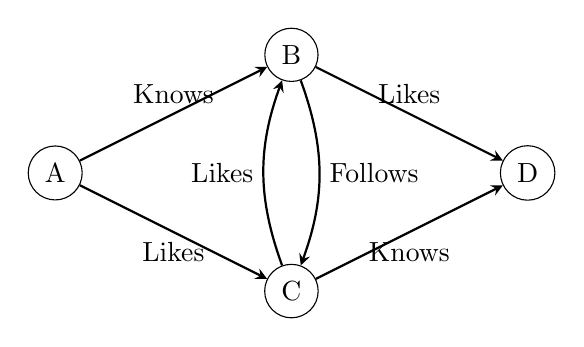
\begin{tikzpicture}[>=stealth]

        % Nodes
        \node[draw, circle] (A) at (0,0) {A};
        \node[draw, circle] (B) at (3,1.5) {B};
        \node[draw, circle] (C) at (3,-1.5) {C};
        \node[draw, circle] (D) at (6,0) {D};

        % Edges
        \draw[->, thick] (A) -- node[above] {Knows} (B);
        \draw[->, thick] (A) -- node[below] {Likes} (C);
        \draw[->, thick] (B) -- node[above] {Likes} (D);
        \draw[->, thick] (C) -- node[below] {Knows} (D);
        \draw[->, thick, bend left=20] (B) to node[right] {Follows} (C);
        \draw[->, thick, bend left=20] (C) to node[left] {Likes} (B);

    \end{tikzpicture}
    \caption{Example graph used throughout this section.}
\end{figure}

Assume the set $S$ contains all paths of length two starting from node $A$:

\[
p_1: A \rightarrow B \rightarrow D
\qquad
p_2: A \rightarrow C \rightarrow D
\qquad
p_3: A \rightarrow B \rightarrow C
\qquad
p_4: A \rightarrow C \rightarrow B
\]

%}
\subsection{Selection}
%{
%\color{blue}
Selection filters a set of paths according to predicates over nodes, edges, or their properties and is defined as follows:

\[
\sigma_c(S) = \{ p \in S \mid c(p) \}
\]

As an example, we filter the path set according to the label of the first edge.

\[
\sigma_{\text{Knows}}(S)=\{p_1,p_3\}
\]

\[
\sigma_{\text{Likes}}(S)=\{p_2,p_4\}
\]

The result is two subsets of $S$, each containing paths that satisfy the corresponding predicate. Unlike graph traversal itself, selection does not modify paths; it only filters the existing path set.
%}

\subsection{Union}
%{
%\color{blue}

Union combines two path sets into a single result.

Using the subsets obtained above,

\[
S_1=\sigma_{\text{Knows}}(S),
\qquad
S_2=\sigma_{\text{Likes}}(S),
\]

their union reconstructs the original path set:

\[
S_1\cup S_2
=
\{p_1,p_2,p_3,p_4\}
=
S.
\]

This illustrates that path sets from different query operations can be combined using the usual set-union semantics.

\subsection{Path Concatenation}
%{
%\color{blue}
Concatenation joins two compatible path fragments into a longer path. Two paths are compatible if the last node of the first path equals the first node of the second path.

Using the running example, we first consider shorter path fragments:

\[
A\rightarrow B,
\qquad
A\rightarrow C,
\]

and

\[
B\rightarrow D,
\qquad
C\rightarrow D.
\]

Concatenating compatible fragments produces longer paths:

\[
(A\rightarrow B)\circ(B\rightarrow D)
=
A\rightarrow B\rightarrow D
=
p_1,
\]

\[
(A\rightarrow C)\circ(C\rightarrow D)
=
A\rightarrow C\rightarrow D
=
p_2.
\]

A query can therefore construct longer paths from smaller path fragments. This is similar to a relational join, but the result is a path rather than a tuple.

\subsection{Closure and Compositionality}
%{
%\color{blue}
A central property of the core algebra is closure: every operator returns another set of paths. Consequently, the output of one operator can immediately serve as the input to another.

In the running example, the selection operator produced the path sets

\[
S_{\text{Knows}}
\quad\text{and}\quad
S_{\text{Likes}},
\]

which could subsequently be combined again using union or further extended using concatenation. Since every intermediate result remains a valid path set, complex path queries can be built from simpler expressions in a modular way.

This compositionality is one of the main strengths of the algebra. It allows query evaluation to be decomposed into reusable intermediate results, supports algebraic query optimization, and provides a clean logical foundation for graph query processing \cite{angles2024path}.
%}
\section{Recursive Path Algebra}

A central requirement of graph query languages is the ability to express recursive navigation over paths of unbounded length. In the path algebra, recursion is represented by the operator $\phi$, which repeatedly applies path concatenation to construct paths of increasing length \cite{angles2024path}.
The recursive operator can be understood as a repeated self-join: starting with a set of paths, it combines the paths with the original set and continues until no new paths are produced. This corresponds to the Kleene plus operation used in regular expressions \cite{angles2024path}.
Intuitively, recursion repeatedly extends short paths into longer ones by concatenating compatible path fragments. Starting from a base set of edges, each iteration adds exactly one additional step, gradually generating longer and more complex paths.


\subsection{Recursive Operator}

Let $S$ be a set of paths. The recursive operator $\phi$ repeatedly joins the paths in $S$ with the paths generated in the previous iteration \cite{angles2024path}:

\[
\phi_0(S) = S
\]

and for $i > 0$,

\[
\phi_i(S)
=
\left(\phi_{i-1}(S) \bowtie S\right)
\cup
\phi_{i-1}(S).
\]

The recursion continues as long as new paths are produced. In other words, the operator starts with the paths in $S$, repeatedly extends them by concatenating paths from $S$, and stops when an iteration does not add any new paths. The resulting operator corresponds to the Kleene plus operation, producing paths of one or more repetitions of the input pattern \cite{angles2024path}.

To illustrate the recursive process, consider the following base set of edges:

\[
S = \{ A \rightarrow B,\; B \rightarrow C,\; C \rightarrow B \}.
\]

The first iteration contains the original edges:

\[
S^{(1)} = \{ AB,\; BC,\; CB \}.
\]

In the next iteration, compatible paths can be concatenated:

\[
S^{(2)}
=
S^{(1)} \bowtie S
=
\{ ABC,\; BCB,\; CBC \}.
\]

A further iteration produces longer paths, for example:

\[
S^{(3)}
=
S^{(2)} \bowtie S
=
\{ ABCB,\; BCBC,\; CBCB \}.
\]

Thus, repeated application of the join operator generates progressively longer paths.

\subsection{Path Semantics}

Graph query languages distinguish between different restrictions on path repetition in order to control expressiveness and computational complexity. These semantics can be modeled as constraint operators applied to the recursive closure:

\begin{itemize}
    \item \textbf{Walk semantics}: no restrictions on node or edge repetition; $\phi$ operates over all finite concatenations.
    \item \textbf{Trail semantics}: edges may not repeat within a path, restricting concatenation to edge-simple expansions.
    \item \textbf{Acyclic semantics}: nodes may not repeat, enforcing cycle-free path construction.
    \item \textbf{Simple path semantics}: no repeated nodes, except that the first and last node may be the same.
    \item \textbf{Shortest path semantics}: selects minimal-length paths from the recursively generated set.
\end{itemize}

%{\color{blue}
Using the example above, the paths in $S^{(3)}$ and $S^{(4)}$ clearly illustrate that recursion over concatenation naturally produces walks. However, at some point some of these walks are no longer trails or simple paths, since nodes such as $B$ and $C$ are revisited multiple times (e.g., $A \rightarrow B \rightarrow C \rightarrow B$). This highlights why additional semantic restrictions are necessary in practical query languages to prevent uncontrolled path growth.


\subsection{Key Issue: Cyclic Graphs and Infinite Expansions}

The main difficulty with recursive path evaluation appears in graphs containing cycles. In such graphs, unrestricted recursion can repeatedly traverse the same cycle and therefore produce infinitely many distinct paths. Although the graph itself is finite, the number of possible walks can be infinite \cite{angles2024path}.

For example, if a path can reach a cycle between two nodes, the recursive operator can continue traversing that cycle and generate paths of increasing length. Under the default walk semantics, the evaluation may therefore never terminate \cite{angles2024path}.

The path semantics introduced above provide a way to control this behavior. Restricting recursion to trails, acyclic paths, simple paths, or shortest paths limits which paths can be generated and can therefore produce finite results on finite graphs \cite{angles2024path}.
\section{Mapping to GQL and SQL/PGQ}

The path algebra can be used to describe path queries from GQL and SQL/PGQ using a common set of operators \cite{angles2024path}. In particular, the path modes of these languages can be represented using recursive operators together with grouping, ordering, and projection. This makes it possible to describe the evaluation of a path query as a sequence of algebraic operations.

\subsection{Selectors and Restrictors}

GQL uses selectors and restrictors to control the paths produced by a path query \cite{angles2024path}:
\begin{itemize}
    \item \textbf{Restrictors}: determine which paths are considered during recursive evaluation, such as WALK, TRAIL, SIMPLE, and ACYCLIC.
    \item \textbf{Selectors}: determine which of the resulting paths are returned, such as ALL, ANY, and ANY SHORTEST.
\end{itemize}

\subsection{Algebraic Encoding}

Each selector-restrictor combination can be expressed using a combination of:

\begin{itemize}
    \item recursion operator ($\phi$),
    \item grouping operator ($\gamma$),
    \item ordering operator ($\tau$),
    \item projection operator ($\pi$).
\end{itemize}

\subsection{Example Translation}

Consider the following GQL query:

\begin{verbatim}
MATCH ANY SHORTEST TRAIL
p = (x)-[:KNOWS]->+(y)
\end{verbatim}

The query asks for one shortest trail between each pair of connected nodes. The
TRAIL restrictor means that edges cannot be repeated, while ANY SHORTEST
selects one shortest path for each source-target pair \cite{angles2024path}.

The corresponding algebraic evaluation can be understood as a sequence of
operations. First, the edges labeled \texttt{KNOWS} are selected. The recursive
operator $\phi_{\text{Trail}}$ then generates paths that satisfy the TRAIL
semantics. The resulting paths are grouped by their source and target nodes,
ordered by path length, and finally projected so that one path is returned from
each group.

In simplified form, the structure of the translation is:

\[
\pi \Big(
    \tau \big(
        \gamma \big(
            \phi_{\text{Trail}}(
                \sigma_{\text{KNOWS}}(\text{Edges}(G))
            )
        \big)
    \big)
\Big).
\]

The exact parameters of $\gamma$, $\tau$, and $\pi$ determine how paths are
grouped, ordered, and selected. This example shows how a GQL path mode can be
represented as a composition of algebraic operators \cite{angles2024path}.

\subsection{Expressiveness}

The path algebra can represent the selector-restrictor combinations defined by
GQL and SQL/PGQ \cite{angles2024path}. At the same time, the algebra allows
additional combinations because grouping, ordering, projection, and recursion
are represented as separate operators.

For example, the algebra can combine a recursive trail operator with grouping
by path length and then select one path from each group. Such a combination is
not directly provided by the GQL path mode syntax \cite{angles2024path}.

The authors show that the different choices of grouping, ordering, projection,
and recursion result in a larger space of possible expressions than the
selector-restrictor combinations defined by GQL. This means that the algebra
is not limited to reproducing existing language features, but can also describe
path operations that are not directly available in the current standards
\cite{angles2024path}.
\section{Relation to Formal Foundations}

The path algebra is related to several established formalisms in database and automata theory. Its operators resemble those of relational algebra, while its recursive operator is closely related to the regular expressions used in regular path queries. Semiring-based approaches provide another point of comparison, since they also use algebraic operations to combine paths.

\subsection{Relation to Relational Algebra}

The path algebra is closely related to relational algebra. Both use operators such as selection ($\sigma$), union ($\cup$), and join ($\bowtie$), but they operate on different kinds of objects. In relational algebra, the operators are applied to relations containing tuples, whereas the path algebra operates on sets of paths \cite{codd1970,angles2024path}.
In the path algebra, selection filters paths according to predicates over their nodes and edges, union combines path sets, and join concatenates compatible paths. The join operation therefore has a different meaning from a traditional relational join, since its result is a longer path rather than a tuple
The main difference is that paths preserve the order and connectivity of the nodes and edges they contain. This makes the path algebra suitable for navigation-oriented queries, where the path itself can be part of the query result.

\subsection{Relation to Automata Theory}

Regular path queries (RPQs) are commonly described using regular expressions over edge labels. These expressions can be translated into finite automata, which can then be used to evaluate whether paths in a graph satisfy the given pattern \cite{mendelzon1995}.

The path algebra describes similar recursive path patterns using algebraic operators. In particular, the recursive operator $\phi$ corresponds to repeated path concatenation and is related to the Kleene plus operation of regular expressions. Zero-length paths can additionally be included when Kleene star semantics are required \cite{angles2024path}.

The two approaches therefore emphasize different aspects of path querying. Automata provide a model for recognizing paths that satisfy a regular expression, while the path algebra describes how sets of paths can be constructed and manipulated using algebraic operators. The approaches are therefore complementary rather than competing formalisms.

\subsection{Relation to Semiring Frameworks}

Semiring-based approaches provide another algebraic way to model path problems. A semiring defines two operations that can be used to combine
alternative paths and to concatenate path weights. Depending on the chosen semiring, this can support tasks such as path counting, shortest-path computation, or probabilistic analysis \cite{rodriguez2011,garcia2022}.

The path algebra shares the idea of using algebraic operations for path composition, but its purpose is different. Instead of assigning a value to each path and aggregating these values, the path algebra treats the paths themselves as query objects. Its operators therefore describe how path sets are constructed, filtered, and combined \cite{angles2024path}.

The two approaches can therefore be viewed as complementary. Semiring frameworks are useful when paths need to be evaluated quantitatively, while the path algebra focuses on the structural and logical representation of path queries.
\section{Discussion}

The path algebra proposed by Angles et al. provides an algebraic framework for describing path queries in graph query languages \cite{angles2024path}. Its main idea is to treat paths as query objects and to define operations for filtering, combining, and recursively extending them.
A key advantage of the algebra is its treatment of paths as first-class objects. Since the operators return sets of paths, the result of one operation can be used as the input to another. This makes it possible to construct complex path queries from smaller algebraic expressions \cite{angles2024path}.
Another important feature is the explicit modeling of recursion through the operator $\phi$. Different variants of the recursive operator can represent walk, trail, acyclic, simple, and shortest-path semantics \cite{angles2024path}.

From a systems perspective, the algebra can serve as a basis for logical query planning. An algebraic expression can be represented as a tree of operations, which makes the individual steps of query evaluation explicit \cite{angles2024path}.
This also creates opportunities for query optimization, for example by changing the order of operations or by applying equivalent algebraic expressions. The actual execution of these plans, however, requires physical operators and cost models that are outside the scope of the proposed algebra.

A limitation of the framework is that it does not define physical execution strategies or cost models. In particular, recursive path evaluation can become expensive on large or highly cyclic graphs. Efficient implementations therefore require physical operators and optimization techniques that are not part of the logical algebra itself.

Despite these limitations, the framework represents an important step toward a standardized and implementation-independent foundation for graph query processing.
\section{Conclusion}

This seminar paper presented the path algebra for graph query languages proposed by Angles et al. \cite{angles2024path}. The algebra treats paths as first-class query objects and provides operators for selection, union, concatenation, and recursion. These operators make it possible to describe path queries in a compositional way.

The paper also examined how the algebra relates to path querying features in GQL and SQL/PGQ, including different path selection and restriction semantics. Furthermore, it was compared with relational algebra, automata-based approaches to regular path queries, and semiring-based models. These comparisons show that the path algebra combines ideas from existing formalisms while focusing specifically on the construction and manipulation of paths.

The main strength of the approach is that it provides a common logical framework for describing different types of path queries. At the same time, the algebra does not specify physical execution strategies or cost models. Efficient evaluation of recursive path queries, especially on large and cyclic graphs, therefore remains an important practical challenge.

Overall, the path algebra provides a useful foundation for reasoning about graph path queries and offers a clear connection between the semantics of modern graph query languages and their underlying algebraic operations.



%\textcolor{blue}{
%\begin{credits}
%\subsubsection{\ackname}
%% The author would like to thank the seminar supervisor for valuable feedback and guidance throughout the preparation of this paper.
%\sout{Not sure if this is needed in this seminar paper.}
%\subsubsection{\discintname}
%\sout{I declare that there are no competing interests relevant to the content of this paper. I am also not sure if this subsubsection is needed in this seminar paper.}
%\end{credits}
%}

%
% ---- Bibliography ----
%
% BibTeX users should specify bibliography style 'splncs04'.
% References will then be sorted and formatted in the correct style.
\bibliographystyle{splncs04}
\bibliography{references.bib}
\end{document}
